\q{6}{Error Probabilities Probably} \\ 

A researcher conducts 1000 of the same hypothesis tests (same null, alternative, and test statistic) with different samples of observed data from a population. Throughout her hypothesis tests, she uses a p-value cutoff of .25. 
\\ \\
Suppose the following is a histogram of the p-values recorded during the conclusion for each of the 1000 hypothesis tests. The bin sizes are all a multiple of .05. 

\begin{center}
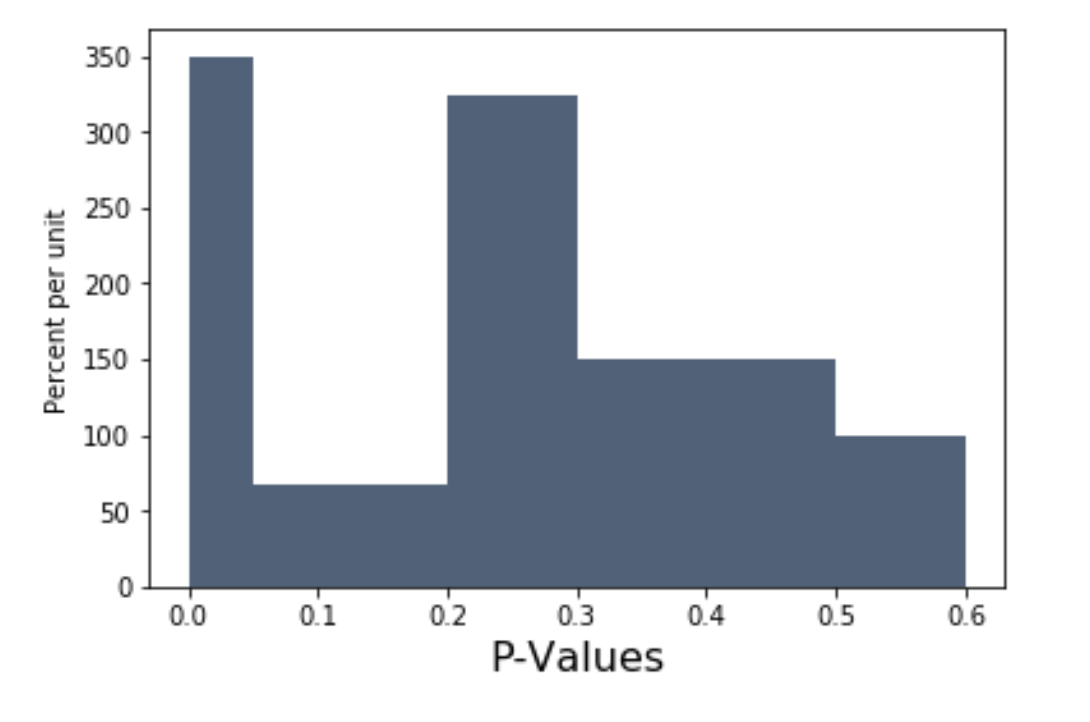
\includegraphics[scale=0.5]{phist.png}
\end{center}

\begin{enumerate}
\subq{3} Assume the null hypothesis in these tests happened to be true. If you can tell, did we reject the null hypothesis more than expected, less than expected, or exactly as many times as we would expect? \textbf{Explain} your answer. If we can not determine with this information, \textbf{explain} why not. 
\begin{itemize}[label=\bubble]
\item More than expected
\item Less than expected
\item Exactly equal to expected
\item Cannot determine
\end{itemize} 
\textbf{Explanation:}
\solution{
	Option 1. With a P-Value cut-off of 25\%, we expect to reject 25\% of all null hypotheses if they were indeed true. Here, we reject at-least $350 * .05 + 60 * .15$ which is greater than 25. 
}
\vfill

\subq{3} Assume the alternative hypothesis in these tests happened to be true. If you can tell, did we fail to reject the null hypothesis more than expected, less than expected, or exactly as many times as we would expect? \textbf{Explain} your answer. If we can not determine with this information, \textbf{explain} why not. 
\begin{itemize}[label=\bubble]
\item More than expected
\item Less than expected
\item Exactly equal to expected
\item Cannot determine
\end{itemize} 
\textbf{Explanation:}
\solution{Option 4. We have no information about anything assuming the alternative hypothesis was true because we never simulated anything under the alternative.}
\vfill
\end{enumerate}



